%%%%%%%%%%%%%%%%%%%%%%%%%%%%%%%%%%%%%%%%%%%%%%%%%%%%%%%%%%%%%%%%%%%%%%%%
% Escuela Politécnica Superior de la Universidad de Alicante
% Realizado por: Jose Manuel Requena Plens
% Contacto: info@jmrplens.com / Telegram:@jmrplens
%%%%%%%%%%%%%%%%%%%%%%%%%%%%%%%%%%%%%%%%%%%%%%%%%%%%%%%%%%%%%%%%%%%%%%%%

\definecolor{mycolor1}{rgb}{1.00000,0.00000,1.00000}%
%
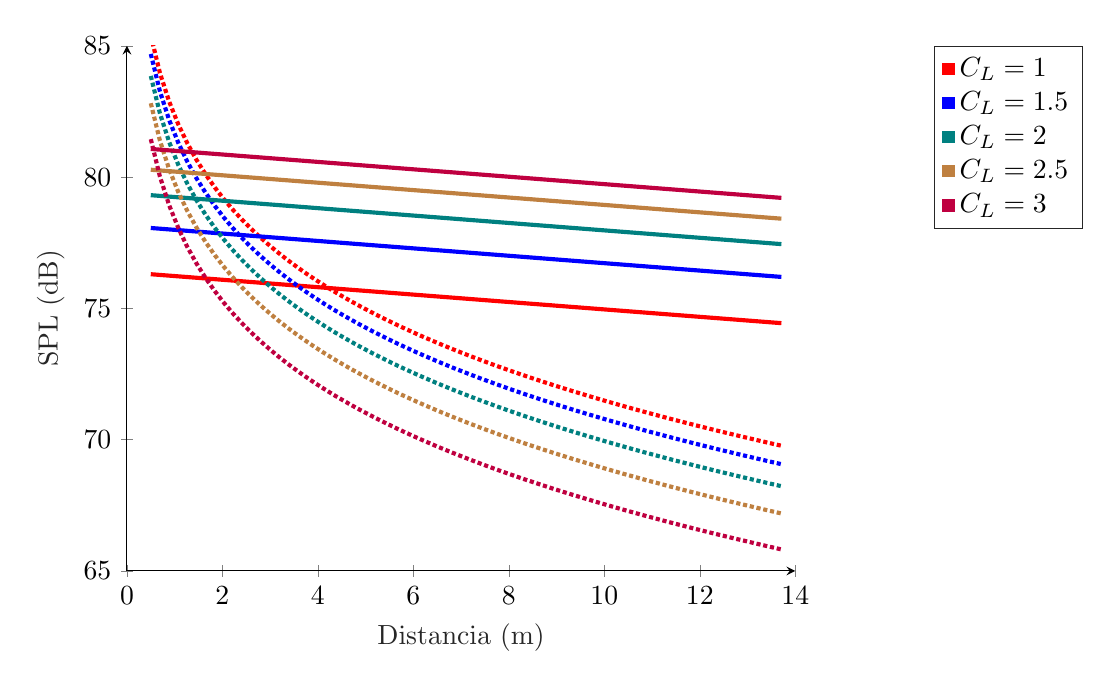
\begin{tikzpicture}

\begin{axis}[%
width=0.7\textwidth,
height=0.55\textwidth,
at={(0\textwidth,0\textwidth)},
scale only axis,
xmin=0,
xmax=14,
xlabel style={font=\color{white!15!black}},
xlabel={Distancia (m)},
ymin=65,
ymax=85,
axis y line=left,
axis x line=bottom,
ylabel style={font=\color{white!15!black}},
ylabel={SPL (dB)},
axis background/.style={fill=white},
legend style={at={(1.43,1)},anchor=north east,legend cell align=left, align=left, draw=white!15!black}
]


% C_E = 1
\def\colorprimero{red}
\addlegendimage{only marks,mark=square*,\colorprimero}
\addlegendentry{$C_L=1$}
\addlegendimage{only marks,mark=square*,blue}
\addlegendentry{$C_L=1.5$}
\addlegendimage{only marks,mark=square*,teal}
\addlegendentry{$C_L=2$}
\addlegendimage{only marks,mark=square*,brown}
\addlegendentry{$C_L=2.5$}
\addlegendimage{only marks,mark=square*,purple}
\addlegendentry{$C_L=3$}
% LATE
\addplot[ color=\colorprimero,line width=1.5,domain=0.5:13.71, samples=10,every node/.style={xshift=-4pt}]
{10*log10(1.0337e+12 * ( (4*0.0026389378)/(1152*(-ln(1-0.1176))) * e^(-(13.82*((x/343)+0.05)*1 / 1.24))*1))};
% EARLY
\addplot[ color=\colorprimero, densely dotted,line width=1.5,domain=0.5:13.71, samples=70,every node/.style={xshift=-4pt}]
{abs(10*log10(1.0337e+12 * (  ( 4*0.0026389378 / (1152*(-ln(1-0.1176))*x) * ( e^(-(13.82*(x/343)*1 / 1.86))*3 - e^(-(13.82*((x/343)+0.05)*1 / 1.86))*1)))))};

% C_E = 1.5
% LATE
\addplot[ color=blue,line width=1.5,domain=0.5:13.71, samples=10,every node/.style={xshift=-4pt}]
{10*log10(1.0337e+12 * ( (4*0.0026389378)/(1152*(-ln(1-0.1176))) * e^(-(13.82*((x/343)+0.05)*1 / 1.24))*1.5))};
% EARLY
\addplot[ color=blue,densely dotted,line width=1.5,domain=0.5:13.71, samples=70,every node/.style={xshift=-4pt}]
{abs(10*log10(1.0337e+12 * (  ( 4*0.0026389378 / (1152*(-ln(1-0.1176))*x) * ( e^(-(13.82*(x/343)*1 / 1.86))*3 - e^(-(13.82*((x/343)+0.05)*1 / 1.86))*1.5)))))};

% C_E = 2
% LATE
\addplot[ color=teal,line width=1.5,domain=0.5:13.71, samples=10,every node/.style={xshift=-4pt}]
{10*log10(1.0337e+12 * ( (4*0.0026389378)/(1152*(-ln(1-0.1176))) * e^(-(13.82*((x/343)+0.05)*1 / 1.24))*2))};
% EARLY
\addplot[ color=teal,densely dotted,line width=1.5,domain=0.5:13.71, samples=70,every node/.style={xshift=-4pt}]
{abs(10*log10(1.0337e+12 * (  ( 4*0.0026389378 / (1152*(-ln(1-0.1176))*x) * ( e^(-(13.82*(x/343)*1 / 1.86))*3 - e^(-(13.82*((x/343)+0.05)*1 / 1.86))*2)))))};

% C_E = 2.5
% LATE
\addplot[ color=brown,line width=1.5,domain=0.5:13.71, samples=10,every node/.style={xshift=-4pt}]
{10*log10(1.0337e+12 * ( (4*0.0026389378)/(1152*(-ln(1-0.1176))) * e^(-(13.82*((x/343)+0.05)*1 / 1.24))*2.5))};
% EARLY
\addplot[ color=brown,densely dotted,line width=1.5,domain=0.5:13.71, samples=70,every node/.style={xshift=-4pt}]
{abs(10*log10(1.0337e+12 * (  ( 4*0.0026389378 / (1152*(-ln(1-0.1176))*x) * ( e^(-(13.82*(x/343)*1 / 1.86))*3- e^(-(13.82*((x/343)+0.05)*1 / 1.86))*2.5)))))};

% C_E = 3
% LATE
\addplot[ color=purple,line width=1.5,domain=0.5:13.71, samples=10,every node/.style={xshift=-4pt}]
{10*log10(1.0337e+12 * ( (4*0.0026389378)/(1152*(-ln(1-0.1176))) * e^(-(13.82*((x/343)+0.05)*1 / 1.24))*3))};
% EARLY
\addplot[ color=purple,densely dotted,line width=1.5,domain=0.5:13.71, samples=70,every node/.style={xshift=-4pt}]
{abs(10*log10(1.0337e+12 * (  ( 4*0.0026389378 / (1152*(-ln(1-0.1176))*x) * ( e^(-(13.82*(x/343)*1 / 1.86))*3 - e^(-(13.82*((x/343)+0.05)*1 / 1.86))*3)))))};


\end{axis}
\end{tikzpicture}%